\documentclass[11pt]{article}

% ---------------------------------------------------------------------------
%  OncoEvidence -- developed proposal (results, tables, figures, math)
%  Compile with:  tectonic docs/proposal_developed.tex
% ---------------------------------------------------------------------------

\usepackage[margin=1in]{geometry}
\usepackage{amsmath,amssymb}
\usepackage{xcolor}
\usepackage{tikz}
\usetikzlibrary{arrows.meta,positioning,fit,backgrounds,calc,shapes.geometric}
\usepackage{booktabs}
\usepackage{array}
\usepackage{colortbl}
\usepackage[most]{tcolorbox}
\usepackage{enumitem}
\usepackage{graphicx}
\usepackage{float}
\graphicspath{{../figures/}{figures/}}

% ----- Palette -------------------------------------------------------------
\definecolor{sriblue}{HTML}{1F4E79}
\definecolor{sriaccent}{HTML}{E8684A}
\definecolor{srigreen}{HTML}{2E8B57}
\definecolor{srigray}{HTML}{4B5563}
\definecolor{srilight}{HTML}{EAF1F8}
\definecolor{sriamber}{HTML}{F6BD16}
\definecolor{srirow}{HTML}{F2F6FB}
\definecolor{srired}{HTML}{C0392B}
\definecolor{nDrug}{HTML}{E8684A}
\definecolor{nGene}{HTML}{2E8B57}
\definecolor{nPath}{HTML}{F6BD16}
\definecolor{nDis}{HTML}{5B8FF9}

\usepackage[colorlinks=true,linkcolor=sriblue,citecolor=sriblue,urlcolor=sriaccent]{hyperref}

\usepackage{titlesec}
\titleformat{\section}{\large\bfseries\color{sriblue}}{\thesection}{0.6em}{}
\titleformat{\subsection}{\normalsize\bfseries\color{sriblue!85!black}}{\thesubsection}{0.5em}{}
\titlespacing*{\section}{0pt}{1.4ex}{0.8ex}

\newtcolorbox{problembox}{colback=srilight,colframe=sriblue,boxrule=0.9pt,
  arc=2pt,left=6pt,right=6pt,top=5pt,bottom=5pt}
\newtcolorbox{winbox}{colback=sriaccent!8,colframe=sriaccent,boxrule=0.9pt,
  arc=2pt,left=6pt,right=6pt,top=5pt,bottom=5pt}
\newtcolorbox{aimbox}[1]{colback=srigreen!7,colframe=srigreen,boxrule=0.8pt,
  arc=2pt,left=6pt,right=6pt,top=4pt,bottom=4pt,title={#1},
  fonttitle=\bfseries\color{white},colbacktitle=srigreen}

\renewcommand{\arraystretch}{1.25}
\newcommand{\NN}{\mathcal{N}}

\begin{document}

\begin{center}
  {\LARGE\bfseries\color{sriblue} OncoEvidence: Mechanism-Guided AI Evidence\\ Triage for Cancer Drug Repurposing}\\[4pt]
  {\large\bfseries\color{sriblue!80!black} Mechanism-grounded AI triage that beats keyword evidence screening on\\ precision and matches expert manual curation at scale}\\[10pt]
  {\large Akshatha Arunkumar}\\[2pt]
  {\small Student Research Institute (SRI), Summer 2026 Cohort \\
  Harvard Undergraduate OpenBio Laboratory}\\[2pt]
  {\small\itshape Developed Proposal \quad\textbar\quad \today}
\end{center}

\vspace{2pt}
\begin{problembox}
\textbf{The problem.} Drug repurposing seeks new uses for existing drugs, for
example whether an approved drug could treat a cancer it was not designed for.
Models can rank thousands of drug-disease pairs, but a score alone is not
actionable: a reviewer needs the \emph{mechanism} (why the drug might work) and
\emph{evidence} (whether the literature supports it). OncoEvidence ranks oncology
candidates, extracts the mechanism path that would explain each one, and uses a
language model to verify that mechanism against published abstracts.
\end{problembox}

\begin{winbox}
\textbf{Thesis.} The contribution is a \emph{methodology comparison}, not a single
model. \emph{Mechanism-grounded AI triage} (knowledge-graph mechanism extraction
plus a literature-grounded language model) is measured against the two status-quo
ways to vet repurposing candidates: a manual / expert-curated process, and naive
automated screening.
\begin{itemize}[leftmargin=1.3em,itemsep=1pt,topsep=2pt]
\item \textbf{Beats keyword screening.} The language-model verifier identifies real
mechanisms with \textbf{0.857 precision}, versus \textbf{0.591} for keyword /
co-occurrence screening of the same abstracts.
\item \textbf{Matches expert manual curation, automatically.} The extracted
mechanisms agree with the expert-curated DrugMechDB at \textbf{0.802}, reproducing
by pipeline what is normally hand-curated, across hundreds of pairs.
\item \textbf{Honest baseline check.} On the plain link-ranking task a tuned tabular
model (XGBoost) matches or beats the graph network, so the graph earns its place by
producing the traceable \emph{mechanism} a tabular model cannot, not by the score.
Mechanism paths separate true from random indications at \textbf{AUROC 0.879}.
\end{itemize}
\end{winbox}

% ===========================================================================
\section{Background and Significance}

Developing a new drug takes many years and large cost, while thousands of approved
drugs already have known safety profiles. If an approved drug acts on a protein or
pathway that also drives a cancer, it can be a fast route to a new treatment.
Biomedical knowledge graphs such as PrimeKG encode millions of relationships among
drugs, proteins, genes, pathways, and diseases, so the information needed to reason
about such mechanisms exists as paths through the graph. The open problem is
\emph{trust}: a bare drug-disease score hides its reasoning, and cannot separate a
real mechanism from a coincidence. OncoEvidence addresses this by making the
mechanism explicit and checking it against the literature and a curated database.

% ===========================================================================
\section{Central Question and Specific Aims}

\begin{problembox}
\textbf{Core question.} For cancer drug repurposing, can a biomedical knowledge
graph combined with a literature-grounded language-model agent prioritize
candidates by both predicted therapeutic relevance and mechanistic plausibility,
and when does the graph add value over a strong tabular baseline?
\end{problembox}

\begin{aimbox}{Specific Aims}
\textbf{Aim 1 (Candidate generation).} Rank drug-cancer pairs with a heterogeneous
graph network and a knowledge-graph embedding, against a tuned XGBoost baseline on
identical features; report honestly where the graph helps.\\
\textbf{Aim 2 (Mechanism extraction).} Extract multi-hop
\emph{drug $\rightarrow$ target $\rightarrow$ pathway/cancer-gene $\rightarrow$
cancer} paths, down-weighting promiscuous hubs.\\
\textbf{Aim 3 (Evidence verification).} A language model grades each path
supported / weak / contradicted / unknown over retrieved abstracts, with a verbatim
quote.\\
\textbf{Aim 4 (Evaluation).} Separation of true vs random pairs, agreement with
curated DrugMechDB mechanisms, and verifier precision.
\end{aimbox}

% ===========================================================================
\section{Datasets and System}

\begin{table}[H]
\centering\small
\begin{tabular}{>{\raggedright\arraybackslash}p{0.24\linewidth} >{\raggedright\arraybackslash}p{0.46\linewidth} >{\raggedright\arraybackslash}p{0.22\linewidth}}
\toprule
\rowcolor{sriblue}\color{white}\textbf{Resource} & \color{white}\textbf{Content} & \color{white}\textbf{Role}\\
\midrule
\rowcolor{srirow} PrimeKG & 129{,}312 nodes, 8.1M edges, 50 relation types; 7{,}957 drugs, 17{,}080 diseases (3{,}170 oncology), 9{,}388 indication edges & Ranking + mechanism paths\\
Europe PMC & abstracts and open-access full text via REST & Evidence retrieval\\
\rowcolor{srirow} DrugMechDB & curated drug mechanism-of-action paths (UniProt-keyed) & Mechanism ground truth\\
\bottomrule
\end{tabular}
\caption{Public resources used. PrimeKG supplies the graph; Europe PMC the
evidence; DrugMechDB the curated mechanisms (mapped UniProt $\rightarrow$ HGNC via
mygene.info).}
\label{tab:data}
\end{table}

\begin{figure}[H]
\centering
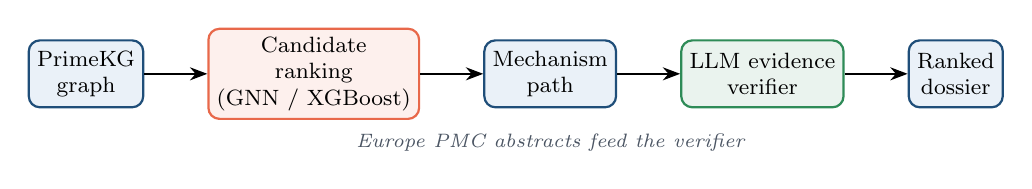
\begin{tikzpicture}[
  node distance=5mm and 8mm,
  box/.style={rounded corners,draw=sriblue,fill=srilight,thick,align=center,font=\footnotesize,inner sep=3pt,minimum height=0.85cm},
  acc/.style={rounded corners,draw=sriaccent,fill=sriaccent!10,thick,align=center,font=\footnotesize,inner sep=3pt,minimum height=0.85cm},
  grn/.style={rounded corners,draw=srigreen,fill=srigreen!10,thick,align=center,font=\footnotesize,inner sep=3pt,minimum height=0.85cm},
  >={Stealth[length=2.2mm]}]
  \node[box] (kg) {PrimeKG\\graph};
  \node[acc,right=of kg] (rank) {Candidate\\ranking\\(GNN / XGBoost)};
  \node[box,right=of rank] (mech) {Mechanism\\path};
  \node[grn,right=of mech] (llm) {LLM evidence\\verifier};
  \node[box,right=of llm] (out) {Ranked\\dossier};
  \draw[->,thick] (kg)--(rank); \draw[->,thick] (rank)--(mech);
  \draw[->,thick] (mech)--(llm); \draw[->,thick] (llm)--(out);
  \node[srigray,font=\scriptsize\itshape,below=2mm of mech] {Europe PMC abstracts feed the verifier};
\end{tikzpicture}
\caption{The OncoEvidence pipeline: rank candidates, extract a mechanism path,
verify it against the literature, output an evidence-backed shortlist.}
\label{fig:pipeline}
\end{figure}

% ===========================================================================
\section{Methods}

\subsection{Candidate ranking and the honest baseline}
Repurposing is framed as link prediction on \emph{drug $\rightarrow$ indication
$\rightarrow$ disease} edges. A heterogeneous graph neural network encodes each
node by message passing over its typed neighbours; with a GraphSAGE-style layer,
\begin{equation}
h_v^{(l)} = \sigma\!\Big( W^{(l)}\big[\,h_v^{(l-1)}\ \big\Vert\
\textstyle\operatorname*{AGG}_{u\in\NN(v)} h_u^{(l-1)}\big]\Big),
\qquad
s(d,c) = \sigma\!\big(z_d^\top R\, z_c\big),
\label{eq:gnn}
\end{equation}
where $s(d,c)$ scores a drug-disease pair. The graph network, a DistMult
knowledge-graph embedding, and a tuned XGBoost baseline all receive the
\emph{same} SentenceTransformer node features, so any gap measures the value of
graph structure, not features.

\subsection{Mechanism-path extraction}
For a candidate we search PrimeKG for short paths through mechanism relations
(drug-target, protein-protein, protein-pathway, protein-disease), scoring each by
specificity and penalizing promiscuous hubs:
\begin{equation}
\mathrm{spec}(x) = \frac{1}{\log_2(\deg(x)+2)},
\qquad
\mathrm{score}(p) = \beta_{\text{type}} + \mathrm{spec}(\text{bridge})\cdot
\frac{1}{\log_2(\delta_{\text{drug}}+2)},
\label{eq:mech}
\end{equation}
where $\delta_{\text{drug}}$ is the number of drugs that bind the bridge protein
(an inverse-frequency penalty that suppresses generic carriers such as albumin),
and $\beta_{\text{type}}$ orders direct-target ($3$) over interaction ($2$) over
shared-pathway ($1$) templates.

\subsection{Evidence verification}
For the top path we retrieve abstracts (a multi-query Europe PMC merge biased
toward mechanism statements), extract the sentences mentioning both the drug and
the target gene, and ask a language model to grade the mechanism as supported /
weak / contradicted / unknown, requiring a verbatim quote and treating a purely
statistical association as \emph{weak}, not supporting.

\subsection{Evaluation metrics}
We report AUROC for separation, agreement with curated mechanisms, and the
precision of ``supported'' verdicts:
\begin{equation}
\text{precision} =
\frac{\#\{\text{``supported'' pairs whose path gene is in the DrugMechDB MOA set}\}}
     {\#\{\text{``supported'' pairs the DrugMechDB covers}\}}.
\label{eq:prec}
\end{equation}

% ===========================================================================
\section{Preliminary Results}

\subsection{Finding 1: the link task does not need the graph}
With a properly tuned XGBoost on shared features, the graph network does not win in
any regime (Table~\ref{tab:bench}). The earlier impression that it did was traced
to an untuned baseline and a message-passing leak, both fixed. We report this
plainly: for link ranking with rich text features, a strong tabular model suffices.

\begin{table}[H]
\centering\small
\begin{tabular}{>{\raggedright\arraybackslash}p{0.34\linewidth} cccc}
\toprule
\rowcolor{sriblue}\color{white}\textbf{Test AUROC (5 seeds)} & \color{white}\textbf{GNN} & \color{white}\textbf{XGBoost} & \color{white}\textbf{MLP} & \color{white}\textbf{KGE}\\
\midrule
\rowcolor{srirow} Transductive & 0.977 & \textbf{0.988} & 0.973 & 0.907\\
Inductive (cold-disease, oncology) & 0.882 & \textbf{0.963} & 0.930 & 0.452\\
\rowcolor{srirow} Inductive (cold-drug) & 0.956 & \textbf{0.958} & 0.931 & 0.482\\
\bottomrule
\end{tabular}
\caption{Corrected benchmark. A tuned XGBoost matches or beats the GNN everywhere;
the DistMult memorizer (KGE) collapses on unseen nodes, confirming the task needs
content features, not memorized identity.}
\label{tab:bench}
\end{table}

\subsection{Finding 2: the graph carries real mechanism}
A tabular model cannot produce a traceable mechanism; the graph can. On true
oncology indications the extractor recovers textbook direct-target mechanisms:
\begin{center}\small\ttfamily
\begin{tabular}{l}
Quizartinib --targets--> FLT3 <--associated-- myeloid leukemia\\
Tamibarotene --targets--> RARA <--associated-- acute promyelocytic leukemia\\
Topotecan --targets--> TOP1 <--associated-- ovarian cancer\\
Trifluridine --targets--> TYMS <--associated-- colorectal cancer\\
\end{tabular}
\end{center}

Over 400 true indications vs 400 random drug-cancer pairs, the mechanism signal
separates the two groups strongly (Table~\ref{tab:sep}, Fig.~\ref{fig:sep}).

\begin{table}[H]
\centering\small
\begin{tabular}{>{\raggedright\arraybackslash}p{0.40\linewidth} cc}
\toprule
\rowcolor{sriblue}\color{white}\textbf{Metric} & \color{white}\textbf{True} & \color{white}\textbf{Random}\\
\midrule
\rowcolor{srirow} Mean mechanism score & \textbf{1.95} & 0.17\\
Direct-target rate & \textbf{34.0\%} & 0.25\%\\
\rowcolor{srirow} Any mechanistic path & \textbf{81.3\%} & 8.8\%\\
\bottomrule
\end{tabular}
\quad
\raisebox{-2.2\height}{\parbox{0.32\linewidth}{\centering\textbf{Separation AUROC}\\[2pt]
{\Large\color{sriaccent}\textbf{0.879}}}}
\caption{Mechanism paths separate true indications from random pairs. A true
indication is roughly $136\times$ more likely to have a direct drug-target to
cancer-gene link than a random pair.}
\label{tab:sep}
\end{table}

\begin{figure}[H]
\centering
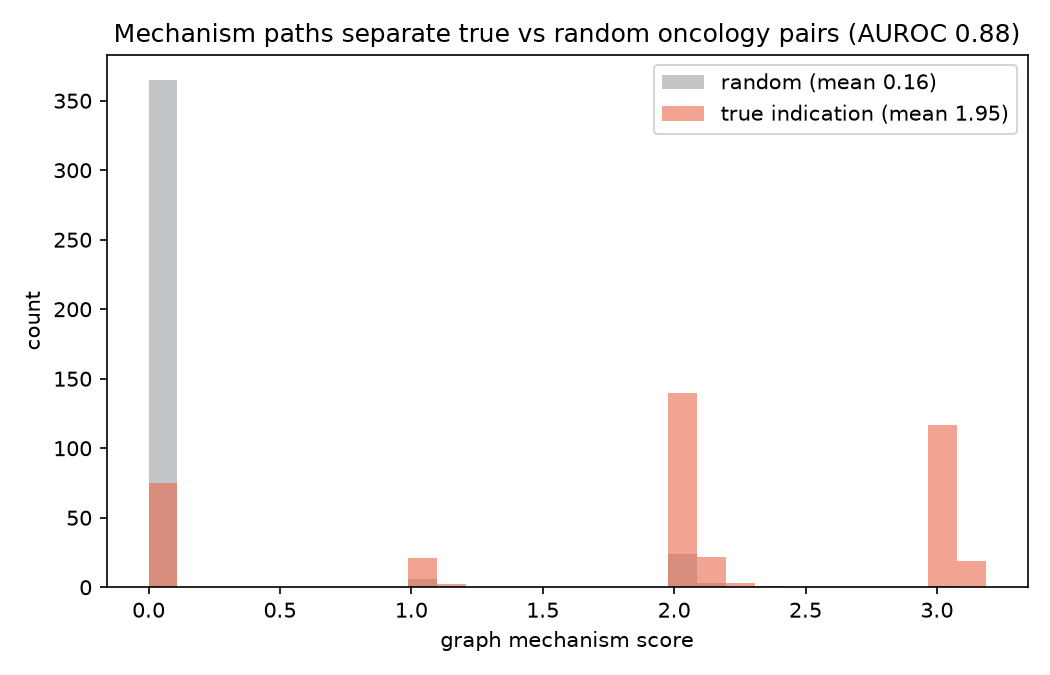
\includegraphics[width=0.78\linewidth]{mechanism_eval.png}
\caption{Distribution of the graph mechanism score for true indications (orange)
vs random drug-cancer pairs (grey). Random pairs pile up at zero; true indications
spread to high, specific scores (AUROC 0.879).}
\label{fig:sep}
\end{figure}

\subsection{Finding 3: the mechanisms agree with a curated database}
Mapping DrugMechDB's UniProt accessions to HGNC symbols makes a direct comparison
possible. On the 263 true pairs DrugMechDB covers, our extracted bridge genes
overlap the curated mechanism genes for \textbf{211 pairs (agreement 0.802)}.

\begin{table}[H]
\centering\small
\begin{tabular}{>{\raggedright\arraybackslash}p{0.30\linewidth} >{\raggedright\arraybackslash}p{0.42\linewidth} c}
\toprule
\rowcolor{sriblue}\color{white}\textbf{Drug} & \color{white}\textbf{Overlapping curated genes} & \color{white}\textbf{}\\
\midrule
\rowcolor{srirow} Methotrexate & ATIC, DHFR, TYMS & \checkmark\\
Topotecan & TOP1 & \checkmark\\
\rowcolor{srirow} Decitabine & DNMT1, DNMT3A & \checkmark\\
\bottomrule
\end{tabular}
\caption{Examples of agreement with curated DrugMechDB mechanisms. DHFR is
methotrexate's canonical target, recovered by the extractor.}
\label{tab:dmdb}
\end{table}

\subsection{Finding 4: the language model verifies precisely}
Run over 50 true vs 50 random pairs, the verifier marks far fewer ``supported''
than a keyword baseline, but those calls are much more trustworthy
(Table~\ref{tab:verify}). A stricter rubric (an explicit drug-to-target statement
is required; a genetic or statistical association is graded weak) plus
sentence-level grounding collapsed ``unknown'' from 14 to 1.

\begin{table}[H]
\centering\small
\begin{tabular}{>{\raggedright\arraybackslash}p{0.34\linewidth} cc}
\toprule
\rowcolor{sriblue}\color{white}\textbf{} & \color{white}\textbf{Language model} & \color{white}\textbf{Keyword baseline}\\
\midrule
\rowcolor{srirow} True pairs graded ``supported'' & 11 / 50 & 34 / 50\\
Random pairs graded ``supported'' & 1 / 50 & 2 / 50\\
\rowcolor{srirow} \textbf{Precision of ``supported'' vs DrugMechDB} & \textbf{0.857} (6/7) & 0.591 (13/22)\\
\bottomrule
\end{tabular}
\caption{The language model is the conservative, precise reviewer: of its
``supported'' calls that DrugMechDB covers, $86\%$ are confirmed, against $59\%$
for keyword matching. Each verdict carries a verbatim quote, e.g. Topotecan / TOP1:
\emph{``a topoisomerase I (TOP1) inhibitor''}.}
\label{tab:verify}
\end{table}

% ===========================================================================
\section{Discussion: what the method beats (and what it does not)}

The contribution is best read as a comparison of three ways to vet cancer
repurposing candidates. Against \emph{keyword / co-occurrence screening}, the
language-model verifier is far more precise (0.857 vs 0.591), because it reads
whether the text actually states a mechanism rather than whether the words merely
co-occur (a keyword screen grades a pharmacogenetic association as ``supported'';
the language model correctly downgrades it to weak). Against the \emph{manual
curation} process, the pipeline reproduces expert DrugMechDB mechanisms at 0.802
automatically and at scale, doing in seconds per candidate what manual literature
review does by hand. We are explicit about what the method does \emph{not} beat: on
the plain link-ranking task a tuned tabular model is as good as the graph, so we do
not claim a model win there; the graph earns its place by producing the traceable
mechanism that a tabular model cannot.

\textbf{Limitations, stated plainly.} We do not claim to beat human experts on
\emph{quality}; we match curated quality while automating and scaling it. The
separation partly reflects that drugs indicated for a cancer already have a known
target linked to that cancer in the graph, so this validates that the graph encodes
\emph{known} mechanism consistently, rather than discovering new biology. Some
metrics rest on modest samples (the verifier precision on seven covered
``supported'' pairs) and partial coverage (DrugMechDB; the open-access full-text
subset). The planned summer work scales the verifier run, broadens full-text
coverage, and applies the same triage to \emph{novel} candidate pairs to generate
mechanism-verified repurposing hypotheses.

% ===========================================================================
\section{Eight-Week Timeline}

\begin{table}[H]
\centering\small
\begin{tabular}{>{\raggedright\arraybackslash}p{0.14\linewidth} >{\raggedright\arraybackslash}p{0.78\linewidth}}
\toprule
\rowcolor{sriblue}\color{white}\textbf{Weeks} & \color{white}\textbf{Milestones}\\
\midrule
\rowcolor{srirow} 1--2 & PrimeKG pipeline; leakage-safe splits; shared features.\\
3--4 & Candidate ranking + tuned XGBoost baseline (Finding 1).\\
\rowcolor{srirow} 5 & Mechanism extraction with hub down-weighting (Findings 2--3).\\
6 & Literature retrieval and the verifier (Finding 4).\\
\rowcolor{srirow} 7 & Full evaluation; scale the verifier; error analysis.\\
8 & Deliverable shortlist, figures, written report.\\
\bottomrule
\end{tabular}
\caption{Weeks 1--6 are already de-risked by the preliminary results above.}
\label{tab:timeline}
\end{table}

% ===========================================================================
\section{Reproducibility and Ethics}

Open tools (PyTorch Geometric, scikit-learn, XGBoost) and public data (PrimeKG,
Europe PMC, DrugMechDB); code, configs, seeds, and the UniProt$\rightarrow$HGNC
cache are released, and every reported number is multi-seed where applicable. All
predictions are research-only and hypothesis-generating, not medical advice.

% ===========================================================================
\begin{thebibliography}{9}
\small
\bibitem{txgnn} Huang K, Chandak P, et al. \textit{A foundation model for
clinician-centered drug repurposing (TxGNN)}. Nature Medicine, 2024.
\bibitem{primekg} Chandak P, Huang K, Zitnik M. \textit{Building a knowledge graph
to enable precision medicine (PrimeKG)}. Scientific Data, 2023.
\bibitem{kgmlxdtd} \textit{KGML-xDTD: a knowledge graph-based framework for drug
treatment prediction and mechanism description}. 2023.
\bibitem{decagon} Zitnik M, Agrawal M, Leskovec J. \textit{Modeling polypharmacy
side effects with graph convolutional networks (Decagon)}. Bioinformatics, 2018.
\bibitem{drugmechdb} Mayers M, et al. \textit{DrugMechDB: a curated database of
drug mechanism paths}. 2022.
\bibitem{sage} Hamilton W, Ying R, Leskovec J. \textit{Inductive representation
learning on large graphs (GraphSAGE)}. NeurIPS, 2017.
\end{thebibliography}

\end{document}
